
%(BEGIN_QUESTION)
% Copyright 2009, Tony R. Kuphaldt, released under the Creative Commons Attribution License (v 1.0)
% This means you may do almost anything with this work of mine, so long as you give me proper credit

The sensor in this diagram is a platinum RTD.  Sketch wires showing how to correctly connect this RTD sensor to the temperature transmitter so that the wire resistance is canceled and will produce absolutely no measurement error:

$$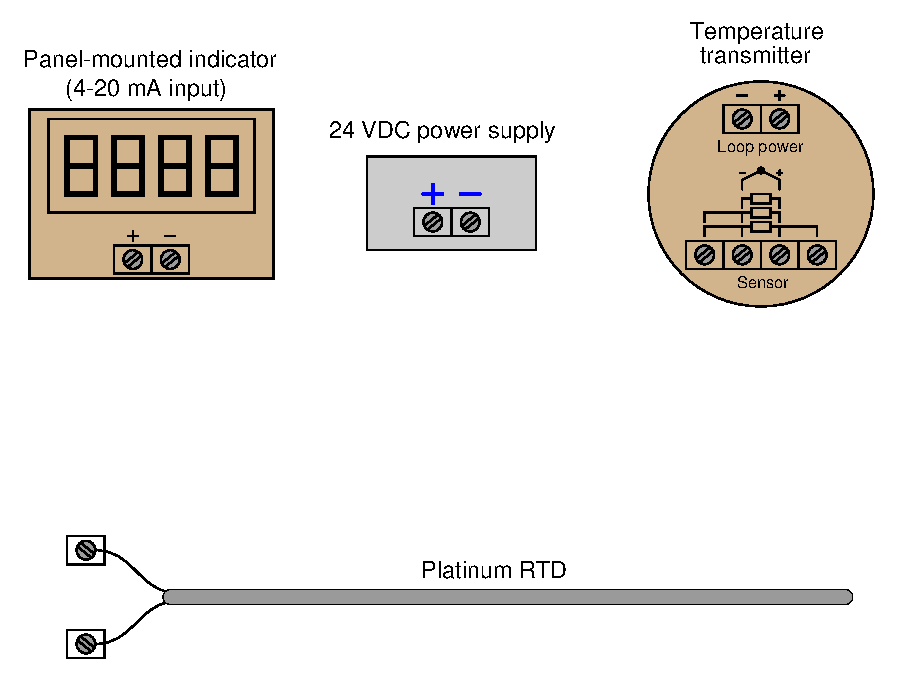
\includegraphics[width=15.5cm]{i04000x01.eps}$$

Note what types of metal each of the connecting wires should be (e.g. copper, chromel, alumel, constantan, iron, platinum, etc.).

\vskip 20pt \vbox{\hrule \hbox{\strut \vrule{} {\bf Suggestions for Socratic discussion} \vrule} \hrule}

\begin{itemize}
\item{} A problem-solving technique useful for making proper connections in pictorial circuit diagrams is to first identify the directions of all DC currents entering and exiting component terminals, as well as the respective voltage polarity marks (+,$-$) for those terminals, based on your knowledge of each component acting either as an electrical {\it source} or an electrical {\it load}.  Discuss and compare how these arrows and polarity marks simplify the task of properly connecting wires between components. 
\item{} Explain how and why the presence of {\it four} wires eliminates wire resistance errors.
\item{} If we were connecting a ``decade box'' precision resistance to the transmitter for the purposes of simulating an RTD at temperature, would we still need to use four wires, or could we get away with using only two wires?
\item{} Suppose all labels and wire colors on the RTD were rubbed off, so you could not even tell what kind of sensor it was: thermocouple, RTD, or thermistor.  Devise a simple test by which you could ascertain the identify of the temperature sensor.
\end{itemize}

\underbar{file i04000}
%(END_QUESTION)





%(BEGIN_ANSWER)

\noindent
{\bf Partial answer:}

\vskip 10pt

The sensor is a two-wire RTD.

%(END_ANSWER)





%(BEGIN_NOTES)

$$\includegraphics[width=15.5cm]{i04000x02.eps}$$

Note: other possibilities for wiring the 4-20 mA ``loop'' circuit exist, but the direction of current needs to be the same as for this circuit.  The excitation/sense wire connections on the RTD may be safely reversed. 

%INDEX% Measurement, temperature: RTD connections

%(END_NOTES)


